\documentclass[11pt]{article}

\usepackage{amsmath}
\usepackage{amssymb}
\usepackage{enumitem}
\usepackage[final]{graphicx}
\graphicspath{{./project_structure.pdf}}

\author{Erik Sturzenhecker, Felix Thiele}
\title{A Start to the formalization of Linear Algebra in ForTheL}

\date{\today}

\begin{document}
\maketitle

\newpage 
\setcounter{tocdepth}{4}
\tableofcontents


\newpage 
\section{Introduction}
\subsection{Naproche}
In this project we build a linear algebra library in ForTheL with Naproche. ForTheL, which stands for Formal Theory Language, is a language that comes close to human language. This reduces many of the initial hurdles people encounter in the formalization of mathematics. Naproche can not only interpret ForTheL code, but is also backed with a strong Automated Theorem Prover, to which we shall refer to as e-prover. This makes many Proofs in our library easier, since some trivial steps can be skipped. At the same time this comes with massive performance issues, since checking this small library is a comparably very time intensive task.

\subsection{Results}
Some of the results given in this library are:
\newline
The \textbf{definitions} of:
\setlist{nolistsep}
\begin{enumerate}[noitemsep]
\item Groups, Rings, Fields
\item Vector spaces, Subspaces, Dual spaces
\item Homomorphisms, Endomorphisms, Automorphisms of vector spaces
\item Lists, Linear independence
\end{enumerate}
And the \textbf{proofs} of:
\setlist{nolistsep}
\begin{enumerate}[noitemsep]
\item A field is a vector space over itself.
\item The linear maps between $K$-vector spaces $V§$ and $W$ form a vector space Hom($K$,$V$,$W$).
\item If $f$ is linear, Ker($f$) is a subspace.
\item If $f$ is linear and Ker($f$) $=$ \{0\}, then $f$ is injective.
\item The endomorphisms of a $K$-vector space $V$ form a ring End($K$,$V$).
\item The invertible elements of a ring form a multiplicative group.
\item Any $K$-vector space $V$ can be embedded into the double dual space $(V^{*})^{*}$
\end{enumerate}

\newpage

\section{Formalization}
\subsection{Project structure}
Giving the project a treelike structure with a file to each topic ensures increased readability and scalability. 
In contrast to having one large file building up mathematics, this enables us to pick what files need to be imported to each file. 
Our structure is depicted in the graph below.

\begin{figure}[h]
\begin{center}
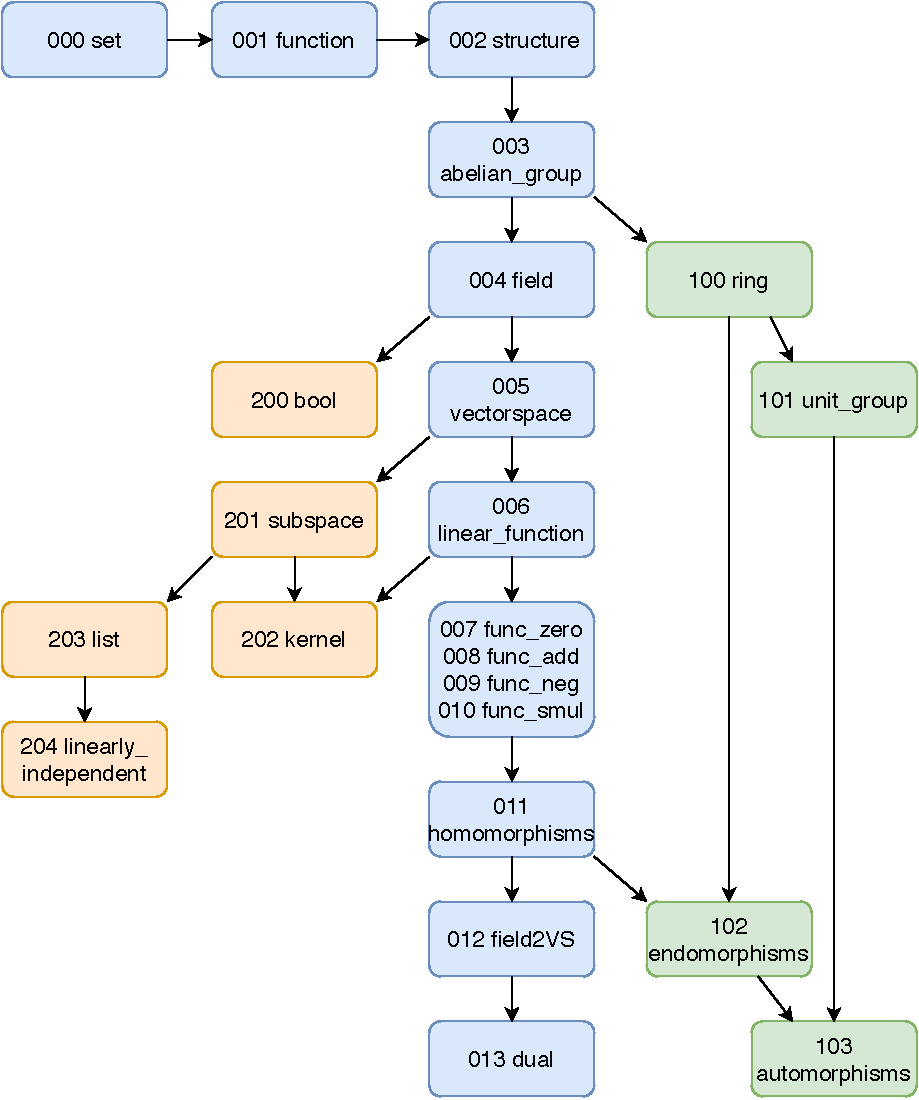
\includegraphics[scale=0.75]{./project_structure.pdf}
\end{center}
\end{figure}

\newpage

The e-prover is not fast enough to compile the entire library with all proofs in reasonable time. 
Instead, for every file we introduce two new files inserting A\_ and P\_ respectively in front of the file names. We insert D\_ before our original file. This gives us an Axiom, Proof and Definition file. 
The Definition file holds all the definitions of the given topic. 
The Proof file holds the theorems and their proofs. The Axiom file holds all the statements of the Proof file in axiomatized form. 
The Proof and Axiom files only read their corresponding Definition file, while Definition files read the Axiom files of all the topics they are building upon. 
This ensures a fast compilation since we don't need to reprove proven statements. 
This structure is depicted below.

\begin{figure}[h]
\begin{center}
\makebox[\linewidth][c]{
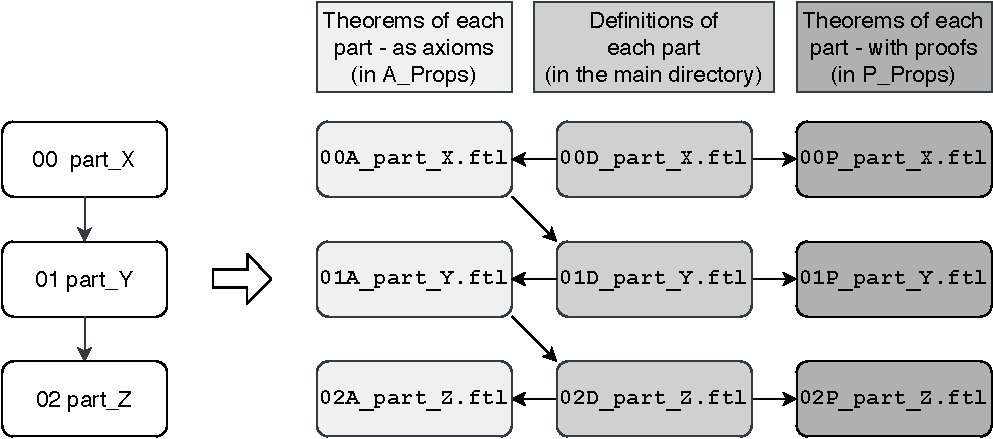
\includegraphics[scale=0.75]{./project_structure_explained.pdf}
}
\end{center}
\end{figure}

\section{Comparison to Lean}


\section{Next Steps in Naproche}


\end{document}

